
\chapter{Methods}
\label{chapter:methods}

In this chapter I discuss computational methods that used throughout my PhD. 
Chief among them is the RNA-seq analysis pipeline. 
My project has consisted of processing large amounts of RNA-seq data and has required a stable workflow that can be run in parallel across multiple computers.
I describe the creation of an RNA-seq library and then each step of the pipeline in detail. 
I then discuss tools for analysing differential gene expression and splicing between conditions.
These provide lists of genes and splicing events but do not by themselves provide biological insight.
It is therefore important to integrate these results with other sources of data.
I describe methods for using RNA-protein interaction data, motif searching, sequence conservation and gene ontology.

\section{Library preparation and sequencing}

RNA-seq involves selecting a pool of RNA molecules and converting them into a sequencing library of complementary DNA (cDNA) fragments. A sequencing machine then samples fragments from this library and convert the sequence of each fragment into digital information. 
It is important to fully understand the steps taken in the preparation of an RNA-seq library when analysing the resulting data. 
Which RNA species are selected, how they are converted and how they are sequenced are all important decisions that will affect the biological questions that can be asked of the data and how the downstream analysis can be carried out.

\subsection{Considerations for the design of RNA-seq experiments}

% Total RNA vs PolyA
RNA sequencing libraries are created from either total cellular RNA (total RNA) or from polyadenylated RNA only.
Total RNA libraries must be depleted of ribosomal RNA species, which consist of 80-90\% of all RNA in the cell \citep{Wilhelm2009}. 
Ribosomal depletion is performed using biotinylated probes that hybridise to ribosomal transcripts. The most popular kit for this is the Ribo-Zero method (Illumina).
In contrast, polyA+ libraries are created  by RNA extraction with poly(Thymine) oligomers which  hybridize to polyadenylated RNA. 
This is sometimes referred to as mRNA-seq, but as multiple non-coding RNAs are polyadenylated this is in fact a misnomer.

Choosing between the two library preparation methods depends on both the biological question of interest but the quality of RNA to be sequenced.
polyA+ RNA-seq has a coverage bias towards the 3\'\ end of transcripts and this is exacerbated when RNA is highly fragmented.  
Total RNA in contrast has a much more even coverage throughout the body of each transcript.
For this reason, total RNA libraries are preferred when working with post-mortem tissue samples due to the high rates of RNA degradation from freeze-thaw cycles in frozen tissue and the effect of formalin on fixed tissue.

When quantifying gene expression, total RNA and polyA+ sequencing libraries are highly concordant \citep{Cui2010,Zhao2018}. 
The effect of 3\'\ bias can be reduced by focusing analysis on the 3\'\ end of transcripts where coverage will be highest. 
%polyA+ libraries made from degraded RNA or certain library preparation kits tend to be highly biased towards coverage towards the 3\'\ end of genes which can confound analyses.
When investigating splicing, total RNA libraries will contain higher proportions of intronic reads, originating from unspliced nascent RNA \citep{Ameur2011}.
This can confound analysis. 
However, total RNA has the benefit of giving information on the expression of a wide range of non-coding RNA transcripts. 
If the user is particularly interested in small RNAs such as microRNAs and small nuceolar RNAs, size fractionation is carried out before sequencing to enrich the library for these species.

For the sequencing itself, there are 4 key considerations: whether single- or paired-end sequencing will be done, whether the library will be stranded,the number of reads sequenced per sample and the length of the reads.
Single- and paired-end sequencing refers to whether one end of the cDNA fragment or both ends will be sequenced.
Stranded libraries retain the direction of transcription for each RNA fragment.
This allows for the discovery of antisense transcripts, such as promoter antisense and 3\'\ antisense transcripts, which are ubiquitious in eukaryotes but poorly understood \citep{Lavorgna2004} and improves quantification of transcripts from genes that overlap from opposing ends. 

These 4 parameters affect the types of analyses that can be performed on the sequencing data.
They also substantially influence the cost of the experiment.
The original 25 base pair unstranded single-end sequencing libraries produced when the technology was in its infancy \citep{Mortazavi2008} are far cheaper than 300bp stranded paired-end, the current maximum with Illumina technology. 

The most obvious measurable outcome is alignment rate - the proportion of sequencing reads that uniquely align to the genome of interest. 
Longer reads increase the unique alignment rate, as do paired-end libraries due to the added constraint on alignment given by both reads in the pair aligning close together. 
For detecting lowly expressed transcripts, sequencing depth is crucial. 
For performing the current state-of-the-art splicing analysis, the most important metric is the number of read that span splice junctions. 
This is less important for the previous generation of software which use exon coverage instead.
With longer reads, the chances of any given read overlapping an intron increase so long (>=100bp) reads are highly recommended.
A study comparing RNA-seq samples at different simulated read lengths recommended 50bp single-end acceptable for differential gene expression and at least 100bp paired-end for splicing \citep{Chhangawala2015}. % depth? recommendations for depth?


\begin{figure}[h!]
	\begin{center}
		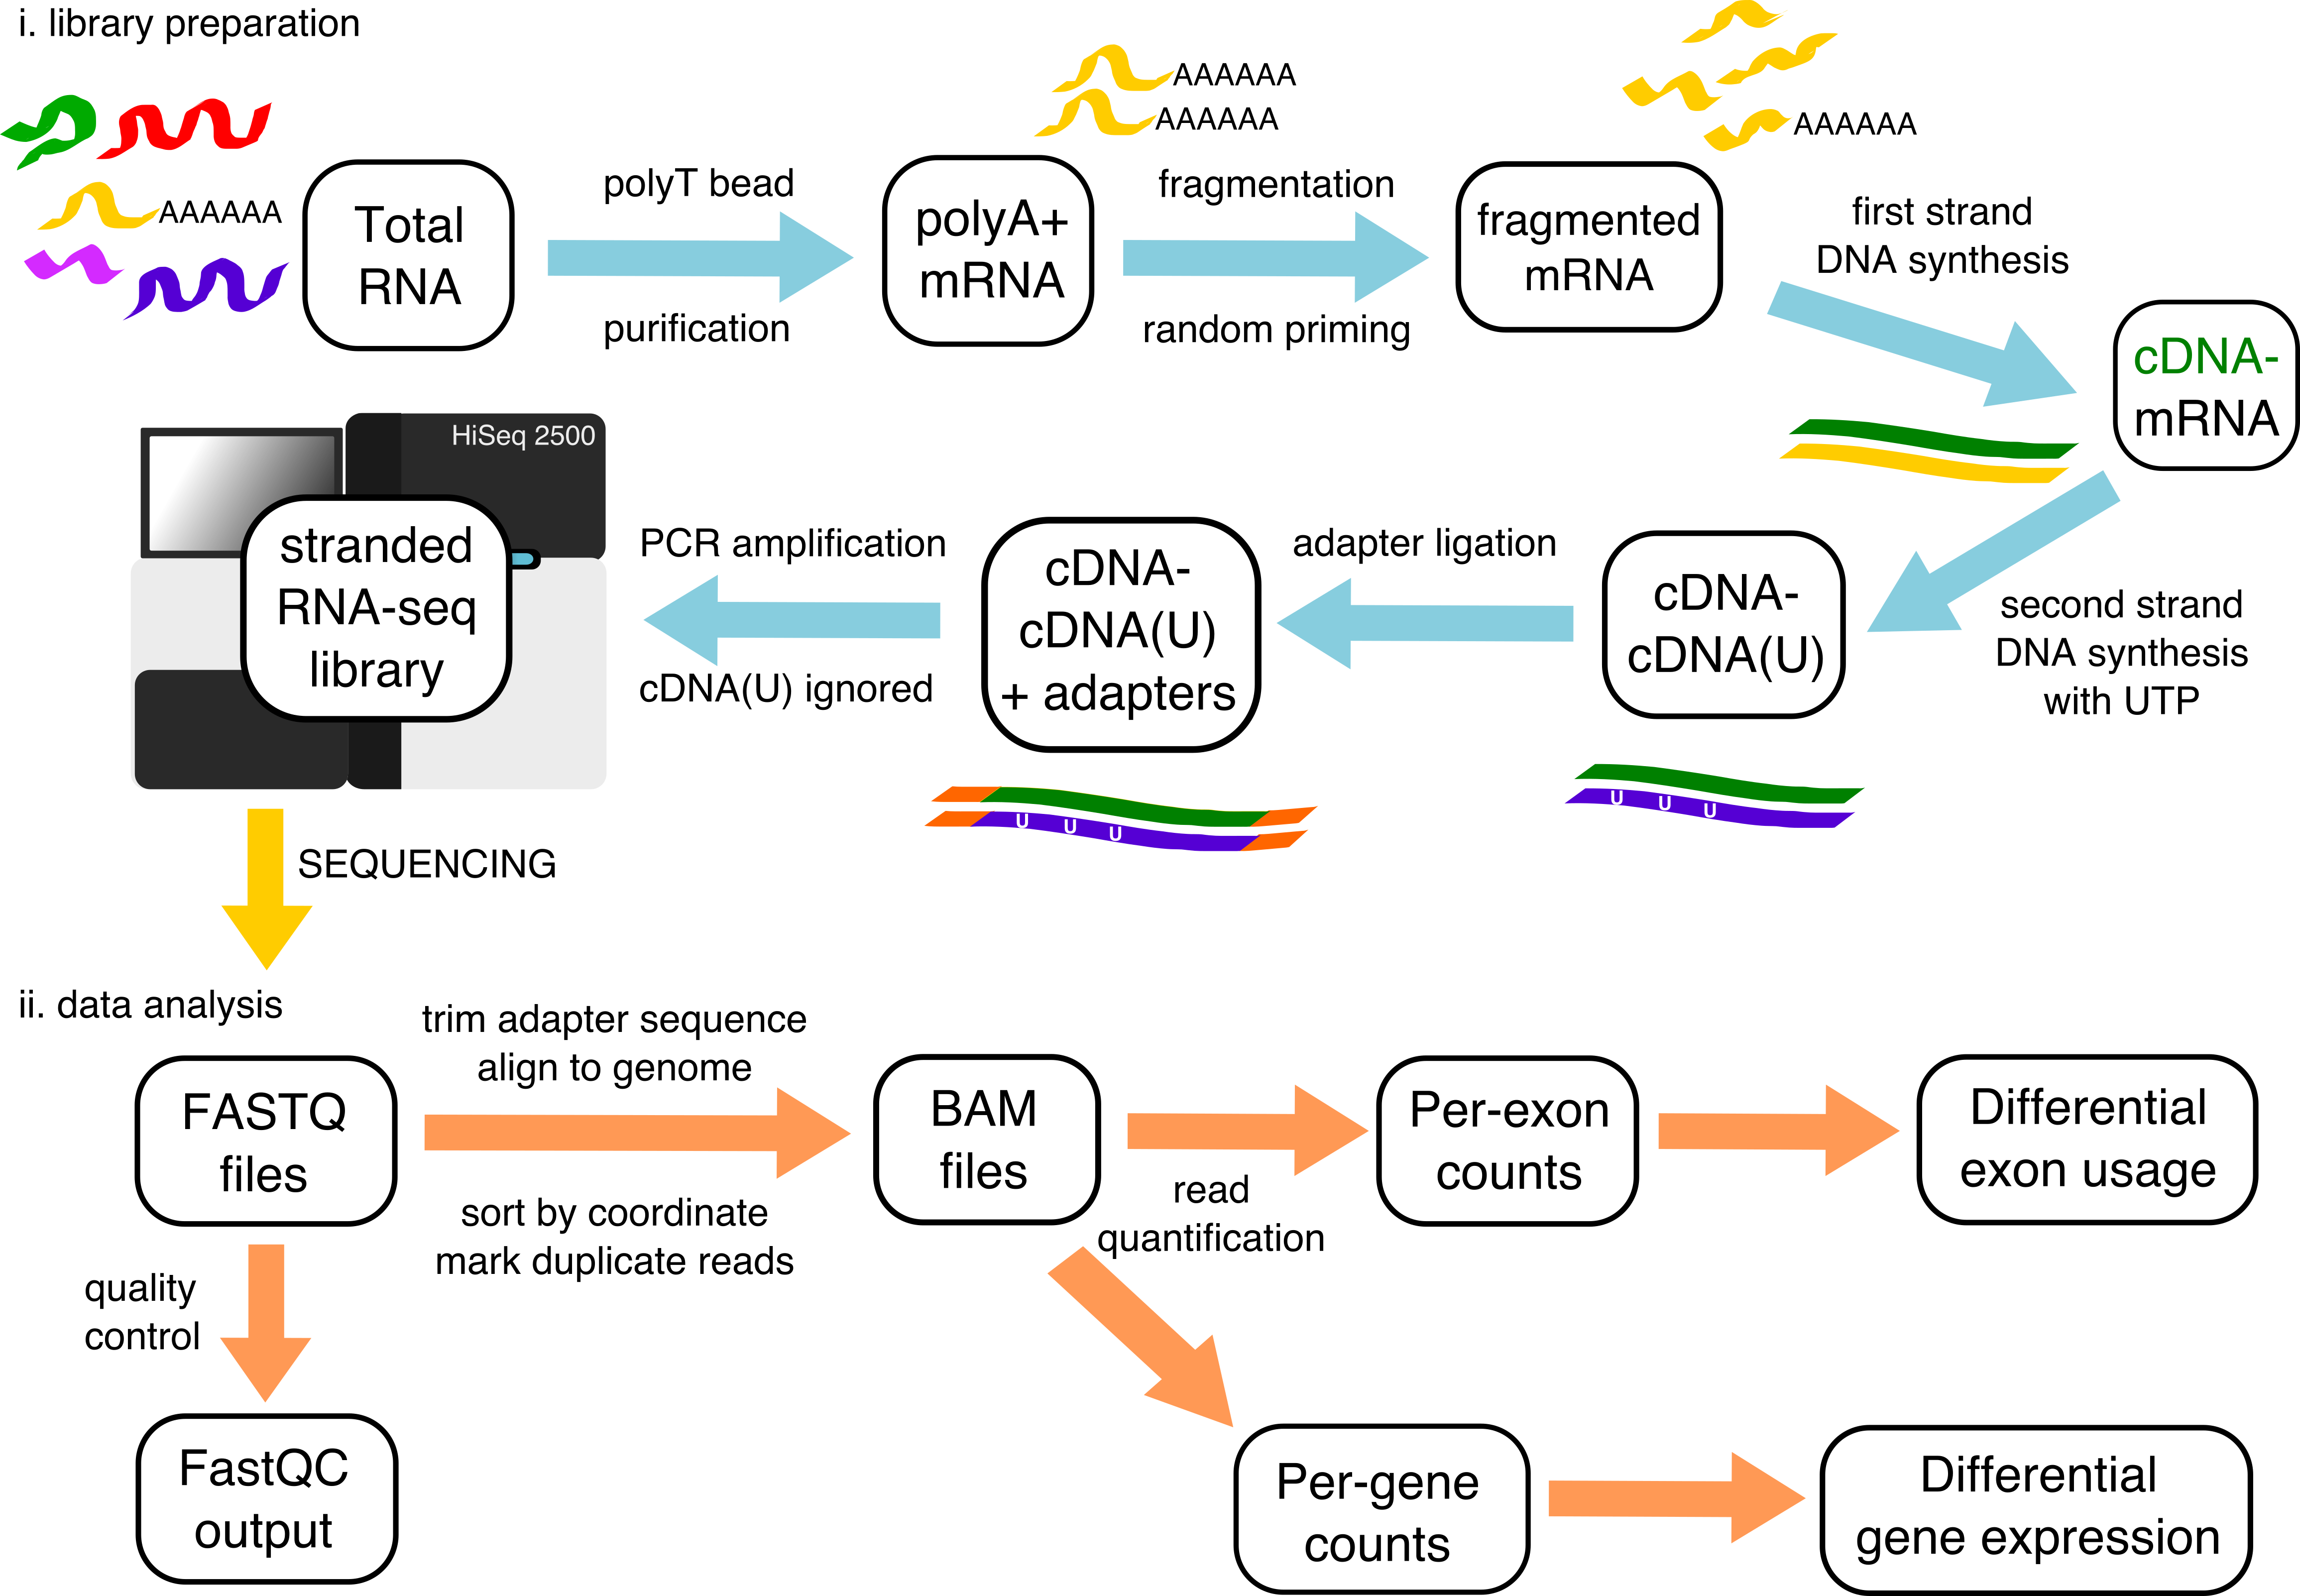
\includegraphics[width=14cm]{Figures/02_methods/RNAseq_pipeline_schematic.png}
	\end{center}
	\caption[Pipeline for stranded RNA-seq preparation and analysis]{
		\textbf{Pipeline for stranded RNA-seq preparation and analysis}\\
	i) Library preparation from total RNA extraction and strand-specific amplification\\
	ii) Bioinformatic analysis workflow to align reads and test for differential gene expression and exon usage
	}
\end{figure}

\subsection{Sequencing library preparation}

The description below is of a polyA+ paired-end and  stranded RNA-seq library preparation for Illumina sequencing.
Total RNA is extracted from cells or tissues using Trizol (Thermo Fisher) or a similar phenol/chloroform reagent \citep{Chomczynski1987}. 
To enrich for mRNA species the RNA is mixed with magnetic beads that are bound to poly(Thymine) oligomers complementary to the poly(Adenine) tail at the 3\'\ end of mRNA. 
The RNA is then fragmented. 
As paired-end sequencing extracts information from each end of the fragment it is important to consider the fragment size in light of the subsequent length of the reads, as with short fragments and long reads the read pairs will overlap leading to redundant information. 
Pseudo-random barcodes are ligated to each fragment to allow for reverse transcription. 
This pseudo-randomness does cause bias towards particular sequences \citep{VanGurp2013}.
The first round of reverse-transcription is carried out forming double stranded DNA-RNA hybrids. 
These complexes are melted and a second reverse-transcription reaction is carried out in the presence of Uracil instead of Thymine, creating double stranded DNA. The Uracilated DNA strand is now in the same orientation as the original mRNA fragment. 
Polymerase chain reaction amplification is then carried out where the uracil containing DNA and the RNA are ignored by the polymerase. 
The resulting library is strand-specific as all the DNA fragments are antisense to the original RNA fragments. Further adapters are added for sequencing in the flowcell and to give the fragments from each sample an identifier as multiple samples are usually pooled together. 
The standard Illumina paired-end sequencing reaction ligates the amplified fragments to wells in the flowcell which then form clusters of identical amplified fragments. 
Sequencing then occurs by sequential addition of fluorescent nucleotides along the length of a fragment in both directions, the  colour of which is recorded by a high resolution sensor. 
This is "sequencing by synthesis", the Solexa/Illumina method \citep{Bentley2008}.
The identity of each nucleotide is determined and given a quality score based on the confidence of the measurement. 
The reads are converted from the basecall (BCL) format to a FASTQ file by the sequencing centre using \textit{bcl2fastq} (Illumina).
The FASTQ file specification \citep{Cock2009} encodes the unique read ID, the read sequence and a quality score. In paired-end sequencing, reads of each pair share a read ID . 
Forward and reverse reads are written into separate files.  
The FASTQ file can be thought of as a digital encoding of the sequences from both ends of each cDNA fragment.

\section{The Plagnol lab RNA-seq pipeline}

A pipeline connects together multiple software tools to convert raw data into summaries and statistics.
Our RNA-seq pipeline converts raw sequencing reads into counts of genes, exons and splice junctions for use in downstream analyses.
This was collaboratively developed by the group of Vincent Plagnol but adapted and occasionally broken by myself.
The pipeline itself is written in the Bash programming language \url{http://www.gnu.org/software/bash/}. 
Individual modules for differential expression and splicing are written in the R statistical programming language \citep{Gentleman1996}. 
Code for the pipeline is freely available to all from (\url{github.com/plagnollab/RNASeq_pipeline/}).

% snakemake and nextflow - better organised, more modular, help with cluster difficulties
The pipeline has been optimised for the UCL Computer Science cluster.
The cluster is made up of hundreds of individual computers or nodes, controlled from a head computer using the Sun Grid Engine system (Univa) for organising and distributing computational work. 
An individual set of instructions to run on a single node is called a job.
This allows for individual steps of the pipeline to be run in parallel or series by distributing steps across multiple jobs.
Jobs can then be linked so that the next step commences once all jobs have completed.
This makes running the pipeline from start to finish as fast and efficient as possible.
However, I have encountered numerous problems while doing my research due to instability and breakages of individual nodes in the cluster.
This can be mitigated by the use of cluster-aware pipeline frameworks such as SnakeMake or NextFlow \citep{Koster2012,DiTommaso2017}. 
These frameworks can restart or reassign jobs when a particular node fails, and increase hardware requirements for nodes when steps repeatedly fail.
I hope that the next version of the pipeline will be written using one of these frameworks.


\subsection{Quality control and read alignment}

% mention multiQC
% talk about QC steps - GC content, random hexamer bias, 3\'\ bias

The first step in any analysis is quality control of the FASTQ files. 
Popular tools like \textit{FastQC} (\url{bioinformatics.babraham.ac.uk/projects/fastqc/}) analyse a set of FASTQ files and produce visualisations of multiple diagnostic tests. 
It can be useful to observe the range of quality scores and how they alter throughout the length of a read to diagnose faults during the sequencing reaction. 
Another important diagnostic is the presence of adapter sequences within reads. 
This can occur when the fragmentation step is too aggressive or when the original RNA sample is heavily degraded, often the case in human post-mortem tissue samples. 
With short fragments, the sequential addition of nucleotides runs into the sequencing adapter sequence, making these reads difficult to align. 
These universal adapter sequences can be removed by software such as \textit{Trim Galore!} (\url{bioinformatics.babraham.ac.uk/projects/trim_galore/}).
This can also remove low quality sequence from the ends of reads, which often occurs towards the end of an Illumina sequencing run. 

Following trimming, the FASTQ files must then be aligned to the genome of the species of interest. 
There have been great advancements in speed and accuracy in alignment algorithms for DNA and RNA. 
The key difference between DNA and RNA alignment is the need for read splitting for RNA. 
As most RNAs are spliced, any cDNA fragment that originates from the boundary between two exons will need to be split and both pieces separately aligned to the genome. 
The interval between two pieces is then recorded by the aligner as a splice junction, the demarcation of where an intron was excised. 
The current state-of-the-art algorithm in both speed and accuracy at resolving splice junctions is \textit{STAR} \citep{Dobin2013-ra}.
\textit{STAR} derives its speed from loading the entire genome into memory and then aligning millions of reads per hour using a seed-and-extend algorithm, where small pieces of each read are aligned and incrementally extended to find the best possible split alignment. 
The alignment information for each read is recorded in a BAM file \citep{Li2009-hm}. 
This format encodes the original read sequence and quality score along information on the alignment, including where the alignment is unique and whether the read was split or clipped by the aligner.
Reads from each pair are initially recorded next to each other and the BAM file is ordered by the read name. 
However for most downstream analyses the BAM file must be re-ordered by genomic position. 
The pipeline does this using the \textit{Novosort} algorithm (\url{http://www.novocraft.com/products/novosort/}). 

If 3\'\ bias is present in a polyA+ RNA-seq library, this can be observed by computing read coverage across all genes with a diagnostic package such as \textit{QoRTS} or RNASeQC \citep{Hartley2015a, Deluca2012}. 
As most differential expression software assumes even coverage throughout a gene body, heavily biased samples can skew the estimates of gene or transcript expression.

For downstream expression analysis, the aligned reads are then quantified for a set of features. These features can either can be whole genes or individual exons. 
There are multiple annotations for the human and mouse genome for known genes and exons are and our pipeline uses the Ensembl transcript annotation as our reference \citep{Cunningham2015}. 
Uniquely aligning reads that overlap each gene or individual exon are counted using \textit{HTSeq} \citep{Anders2015-wz}.

\subsection{Differential gene expression}

The most common application of RNA-seq is for an experiment comparing the abundances of different RNAs between conditions.
This could be for example between the knockdown of a particular gene and a control, or between a group of disease patients and a group of healthy controls. 
These experiments should be made up of multiple biological replicates, where RNA libraries have been prepared from different organisms or cell culture samples under the same conditions. 
This is so a fair assessment can be made of the biological variation in RNA abundance within each condition. 
This is in comparison to technical replicates, where the same library is sequenced multiple times, which can only explain the variance  in the sequencer itself. 
As the concordance between technical RNA-seq replicates is very high \citep{Mortazavi2008}, these are generally shunned in favour of biological replicates. 
RNA-seq is still an expensive experiment and the high cost limits a lab to sequence only a small number of biological replicates to typically less than 5 samples per condition. 
There is also an ethical consideration when working with model organisms on how many samples should be appropriate.
Small sample sizes limit statistical power to detect small variations in RNA abundances and the confidence in the truth of one's results. 
There are multiple algorithms to test for differential expression but we settled on using the \textit{DESeq2} package for its statistical robustness and speed \citep{Love2014}. 
It is desiged to compensate for the small sample sizes used in a typical RNA-seq experiment.

\textit{DESeq2} makes use of the fact that each sequencing library measures the abundance of tens of thousands of transcripts. 
The number of reads generated by each library can be highly variable and so this is also accounted for. 
\textit{DESeq2} normalises the read counts for each gene in each sample by the size of each sample's library, the \textit{size factor}. 
It then assumes that the normalised read counts fit a negative binomial probability distribution. 
It estimates the variance or dispersion in read count for each gene across all samples. 
To compensate for small sample sizes, which give a very high estimate of dispersion, it compares the dispersion between all genes and shrinks each estimate to a local average based on genes expressed at a similar level. 
Using these shrunken dispersion estimates, the software then fits two generalised linear models: a null model where condition has no effect and an alternative model where the change in condition explains the change in gene expression. 
The two models are compared with a Wald test on which model fits the data better, computing a P-value. 
The P-values generated for each gene are adjusted to correct for multiple testing using the Benjamini-Hochberg procedure \citep{Benjamini1995}. 
The output of a differential expression analysis gives both an adjusted P value for each gene and a fitted $log_2$ of the fold change in expression between the two conditions. 
This gives an estimate of the effect size. 
Fold-changes on the $log_2$ scale have the useful aesthetic property of being symmetrical around positive and negative powers of two.
Therefore a doubling of expression will have a $log_2$ fold change of $1$, and a halving will have a $log_2$ fold change of $-1$.


\section{Differential splicing}

Differential splicing is an analysis that looks for changes in splicing between conditions. 
How this is done depends on the frame of reference used. 
I will discuss examples of different approaches.

Generally, methods for differential splicing have followed the increasing sophistication and reducing cost of sequencing technology.
Increases in read length and and greater depth of sequencing due to plummeting sequencing costs have driven the development of new software. These have  made use of the increasing availability of splice junction reads within samples.

I can group software packages into one of four categories based on what they consider to be the fundamental unit of differential splicing. 
All these modern packages work best with high depth paired-end data.
The approaches based on junction reads also require long reads to maximise the information available.

\subsection{Exon quantifiers}

These packages focus on the change in usage of particular exons between conditions. Therefore the fundamental unit of analysis is the exon.
They test for differences in the usage of a particular exon as a ratio of read counts for each exon against all exons. 
This adjusts for differences in baseline gene expression between conditions. 
This approach was first used in the \textit{DEXSeq} package \citep{Anders2012}. 
\textit{DEXSeq} requires a flattened list of "union exons" which is a set of non-overlapping intervals formed from collapsing exons from overlapping transcripts together.
RNA-seq seq reads can then be counted at each union exon. 
This method does not require splice junctions so lower depth and shorter read libraries can be used.
\textit{DEXSeq} normalises the per-exon counts to a library \textit{size factor} and compares the  normalised counts from each exon with the counts from all the exons in a gene.
It then fits a generalised linear model to compare the ratio of exon usage between biological conditions and estimates a fold-change, which is shrunken with a Bayesian shrinkage procedure.
The output of a \textit{DEXSeq} analysis is each union exon in a gene is given a $log_2$ fold change between conditions and an adjusted P value from the test. 
Although this can be used to demonstrate whether differential exon usage occurs due to a condition, it is inherently difficult to extract meaningful information about the underlying biology. 
A significant union exon may not correspond to real exon. 
As they consider the whole gene they are sensitive to poorly annotated genes and extreme biases in coverage.
Therefore, hits from \textit{DEXSeq} need to be closely analysed in the context of the gene they reside in. 
This approach is also dependent on transcript annotation so cannot pick up novel events.
\textit{DEXSeq} has been adapted to look at differential intron usage \citep{Li2015a}.
This work directly inspired my work on \textit{Cryptex}, a software pipeline for using splice junction reads to find novel exons which I discuss in \autoref{chapter:cryptic_exons}.
The intepretability problem has been reduced by a software package called \textit{JunctionSeq} \citep{Hartley2015}, which also quantifies splice junctions and can pick up novel junctions, but uses a DEXSeq framework for differential usage.

\subsubsection{Transcript quantifiers}

Here, the fundamental unit is the transcript. Genes can have many different transcripts which may be highly similar in exon content.
These tools estimate the abundance of different transcripts and compare abundances between conditions.
Transcript assembly algorithms like \textit{RSEM} \citep{Li2011}, \textit{Cufflinks} \citep{Trapnell2010} and \textit{Stringtie} \citep{Pertea2015} assemble aligned reads into transcripts using annotation but also find novel transcripts.
Pseudoaligners like \textit{Kallisto} \citep{Bray2016} and \textit{Salmon} \citep{Patro2017} can work straight from the FASTQ files without prior alignment.  
All these algorithms require long reads for enough splicing information and very dependent on the list of transcripts they are given. 
Some genes can generate hundreds of very similar transcript isoforms or overlap with other genes and so these methods will struggle to accurately assign reads correctly.
\citep{Zhang2017} compared isoform estimation between pseudoalignment tools to alignment-dependent tools (\textit{RSEM}, \textit{Cufflinks}) and found the alignment free methods outpeformed in both speed and accuracy.


\subsection{Local splicing event quantifiers}

A compromise between the two previously mentioned, these methods take the splicing event as fundamental unit and compare changes in inclusion of a splicing event between conditions. 
This relies on the presence of reads that span splice junctions and so require high depth and long reads.
The power of the splice junction rests in its ability to exactly demarcate where an intron has been excised from a transcript. 
The coordinates and counts of each splice junction can then be used to construct and quantify different types of splicing events.
Using this information in analysis provides a much more accurate picture of splicing beyond exon quantifiers which only assess changes in read coverage across exons.
The trade-off is that as splice junction reads are the minority of all reads there is reduced power to detect differential splicing events compared to exon quantification methods.

Typically, splicing events are discovered and classified by constructing a graph database from splice junction reads.
This models splicing events as a set of overlapping nodes and edges. 
The topology of the graph then determines the type of splicing event.
These events may be cassette exons, alternate splice sites, intron retention, mutually exclusive exons or alternate starts and ends. 
This classification greatly aids downstream interpretation as different categories of event may be regulated by different mechanisms.
 Each event is then tested for differences in inclusion/exclusion across conditions. 
 This approach has been implemented in the \textit{SGSeq}, \textit{SUPPA}, \textit{rMATs}, \textit{JUM}, \textit{MAJIQ} and \textit{Whippet} packages \citep{Goldstein2016,Alamancos2015,Vaquero-Garcia2016,Wang2018a,Shen2014, Sterne-Weiler2018a}. 
SGSeq has the unique ability to find novel events not present in annotation. 
It discovers and classifies events and then provides counts reads supporting inclusion and exclusion of each event.
These counts are then fed into the \textit{DEXSeq} framework and a general linear model fitted to test the effect of condition. % do the others? don't think so. 
\textit{Whippet} combines features of the pseudoaligners with the local event quantifiers. 
It first builds an index of splicing events from transcript annotation and then aligns reads to the index straight from the FASTQ file. 
This approach cannot detect novel splicing junctions but can discover novel arrangements of known exons.
All these packages, while providing a clear output of different splicing events, struggle to determine splicing events such as tandem 3\'\ UTR changes which can only be differentiated by read coverage and not splice junctions.
There has been no comprehensive comparison of all these methods to assess which performs best on simulated data.

\subsection{Annotation-free quantifiers}
The fourth and final class of algorithm don't depend on any transcript annotation at all. The \textit{derFinder} package \citep{Collado-Torres2017} assesses changes in read coverage between samples, which is particularly useful in looking for novel non-coding RNA species or in the aforementioned tandem 3\'\ UTR problem. The \textit{LeafCutter} package \citep{Li2016} looks for differentially used splice junctions independently of annotation and has shown that across a set of tissues around 30\% of the high confidence splice junctions recovered are novel to any annotation database. 

% Which tools used in which chapters

\subsection{Deciding on which tools for use for each project}

One of the analytical priorities for my work on TDP-43 and FUS has been to quantify novel splicing changes. These are splicing changes that are not recorded in annotation databases. In \autoref{chapter:cryptic_exons} I developed my own tool to look at cryptic splicing without requiring long reads, as I reanalysed older RNA-seq data. 
The idea behind \textit{CryptEx} was that with shorter reads there are very few splice junctions in an individual sample but by first combining all samples together, novel exons can be discovered and distinguished from random intronic read coverage. 
Once those exons are then determined, the total read coverage over that position can be used to test for differential usage using \textit{DEXSeq}. 
Since that project was published there has been a movement in the field towards tools that can accurately quantify novel splicing but the requirement for read length is still present.
This is now less of a problem as read lengths of 100bp and greater are now routine.

For the work on TDP-43 mutant mice described in \autoref{chapter:tdp_mice}, I used different splicing methods to match the quality of the data, which was generated over 5 years with different generations of library preparation and sequencing technology. For the oldest data, generated from mouse embryonic fibroblasts and head samples with low read depth and short length, I used the DEXSeq package to estimate differential exon usage and \textit{CryptEx} to find novel exons (not included in chapter).
With the newer data from mouse embryonic spinal cord, sequenced with longer paired-end reads and at higher depth, I wanted to local splicing event quantified to take advantage of the high proportion of splice junction spanning reads. 
I chose the \textit{SGSeq} package as it could quantify splicing events from BAM files and used a graph database approach to find novel splicing events as well as classify annotated splicing events. This provided a much richer dataset to work with than the previous \textit{DEXSeq} method.
For my work on combining FUS datasets from multiple groups I again used \textit{SGSeq} for splicing analysis as it uses DEXSeq for statistical testing of splicing event usage between conditions. The general linear model framework provided by DEXSeq allowed me to add dataset-specific covariates and analyse all samples jointly.


%% rewrite - originally from TDP mice chapter
%RNA sequencing allows for unambiguous assignment of splice events in the form of spliced junction reads. 
%However, due to their rare occurrence compared to non junction-spanning reads, the number of junction reads detected in a sample and therefore the power to resolve differential splicing depends on the initial depth of sequencing, the length of sequencing reads and the expression level of the gene. Therefore for low depth sequencing data it is practical to instead infer splicing changes from quantifying read coverage across each exon and ignore junction information. This approach is exemplified by the DEXSeq package \citep{Anders2012} which we used to estimate splicing changes in the embryonic fibroblast and head samples.
%
%When sequencing depth and read length is increased it is possible to more accurately measure splicing variation with spliced junction reads alone. The cassette exon is a splicing variant comprised of three spliced junction reads: two flanking junctions that connect the flanking exons to the central cassette exon and a single parent junction that excludes it. By taking the ratio of the inclusion junction counts over the total number of junctions we can estimate the percent spliced in (PSI) of the cassette exon \citep{Katz2010-ir}. By comparing samples across conditions we can estimate a $\Delta$PSI - the difference in PSI between cases and controls. A positive $\Delta$PSI indicates increased exon inclusion and negative $\Delta$PSI indicates increased exon skipping. 
%
%Due the high depth and long read length of the RRM2mut embryonic brain and LCDmut adult spinal cord samples we used the SGSeq package \citep{Goldstein2016}. This creates a local splicing graph of connected spliced junction reads and determines the splicing events contained within. These events consist of cassette exons, retained introns, alternate $3\'\$ and $5'$ junctions, alternate first and last exons, and mutually exclusive exons and SGSeq allows for the possibility of multiple classes of splicing event to occur within  the same interval. SGSeq  then quantifies  the number of  reads in each sample  that support each splice event and these counts can be used with DEXSeq. 
%
%Due to the current interest in unannotated (novel or cryptic) splicing events, particularly those linked to TDP-43 depletion \citep{Humphrey2017, Ling2015}, there is a need for tools that identify and classify spliced junction reads that cannot be assigned to known transcripts. 


% rMATs insists on all samples having the same read length - what about soft clipping? adaptor trimming? Combining multiple datasets?

\section{Functional analyses}

Downstream of differential expression and splicing analysis, I have used other sources of data to find and understand potential causes and mechanisms for the changes I detect.

\subsection{RNA-protein interaction data}

RNA-binding proteins like TDP-43 and FUS bind to specific RNA sequence motifs in sets of target transcripts.
This binding influences the expression and splicing of these transcripts.
These binding preferences and targets can be observed experimentally using UV crosslinking and immunoprecipitation, or CLIP. 
This uses a specific wavelength of ultraviolet light to form crosslinks, covalent bonds between amino acids and nucleotides in close proximity \citep{Ule2003}. 
These RNA-protein complexes are then purified using an antibody to the protein of interest.
The overhanging RNA and protein is then digested, leaving only a small polypeptide bound to a short fragment of RNA.
The RNA is then reverse-transcribed and sequenced.
With the advent of next-generation sequencing, this was taken transcriptome-wide with the development of high-throughput CLIP (HITS-CLIP) \citep{Licatalosi2008}.
However, CLIP does not provide precise information on which nucleotides in the fragment are bound, as the method depends on the reverse transcriptase reading past the crosslink nucleotide.
As the reverse transcriptase more often than not stalls at the crosslinking position, this can be exploited.
By capturing these truncated cDNAs, the position of the UV crosslink can be determined from the nucleotide directly upstream of where the cDNA aligns to the genome.
This technique, individual nucleotide CLIP or iCLIP, allows for the precise binding sites of a protein to be discovered \citep{Konig2010,Huppertz2014-ip}.
Once the libraries are sequenced and the reads aligned to the genome, unique cDNAs are found by removing duplicate reads and then counted. 
Binding regions are determined with a shuffling procedure which clusters reads within a set distance and compares the counts of each cluster to a shuffled control within the same genomic feature \citep{Wang2010}.
This produces lists of clusters and their component peaks discovered at a false discovery rate of 5\%.
The processing of iCLIP data used in my work was done by the iCOUNT server, maintained by Toma{\v{z}} Curk and colleagues \citep{Curk2016}.

An alternative to iCLIP, enhanced CLIP (eCLIP), reduces the number of PCR duplicate reads in the library  \citep{Van_Nostrand2016-su}. 
eCLIP was used by the ENCODE consortium to profile multiple RNA-binding proteins. 
Data for enriched peaks and clusters is processed and freely available at \url{https://www.encodeproject.org/}. 
Unlike iCLIP, eCLIP does not include a verification step where the correct size of RNA-protein complex is checked by eye.
Therefore one cannot be sure that the cDNA libraries are not from RNAs that interact with other co-purified proteins \citep{Chakrabarti2018}.

I can integrate eCLIP and iCLIP data with my RNA-seq results to correlate binding of RNA targets with changes in gene expression and splicing.
RNA maps are a powerful visulisation tool first used to profile the protein NOVA \citep{Ule2006}.
They plot the distribution of CLIP tags or reads across a set of genomic features.
Typically these features are cassette exons from RNA-seq that are either included or skipped more when the protein of interest is perturbed.
By comparing a set of altered events to a control set of no changes, it is possible to see the scale of enrichment for binding within a particular region. 
This has been used to show positional specificity around splice sites for multiple RNA-binding proteins \citep{Ule2006, Wang2010,Konig2010}.
As well as constructing RNA maps, I have used iCLIP and eCLIP data to look at CLIP binding on different types of genomic features, such as introns and 3\'\ untranslated regions.

CLIP-based methods do not provide an absolute measure of binding affinity between a protein and its target RNAs. 
The number of unique overlapping cDNA reads at a position is a combination of the binding affinity at that position and the underlying expression of the target.
It is not possible therefore to distinguish high affinity binding from low affinity binding. 
Direct comparisons of cDNA counts between CLIP profiles of the same protein under different conditions are therefore difficult to make.
In addition, data can only be generated from sites that are both expressed in the cell type tested and can be aligned to the genome. 
The latter precludes the use of CLIP methods on understanding binding to repetitive regions within specific genes \citep{Chakrabarti2018}.
There are also inherent technical biases in UV crosslinking and RNase digestion that affect the cDNA profile.
Despite these caveats, CLIP-based methods, in combination with RNA-seq, are powerful tools for improving our understanding of RNA biology.

\subsection{Functional annotation with ontologies}

High throughput analyses can produce large lists of genes.
Understanding how these genes fall into specific functional sets and/or pathways provides important biological insight.

The Gene Ontology (GO) initiative seeks to annotate every gene with function information \citep{Ashburner2000,Carbon2017}.
GO terms are split into three domains: molecular function, cellular component and biological process. 
Terms have defined relationships with each other in a hierarchical structure; more specific terms are the children of broader terms.
The Kyoto Encyclopedia of Genes and Genomes (KEGG) annotates genes to pathways of interacting molecules as well as to sets of genes linked to particular human diseases \citep{Ogata1999}.
Both databases share experimental information across orthologous genes between species.
Annotations may be from direct experimental evidence or inferred through computational methods such as protein sequence and structure comparison, which make up the majority of annotations as of 2010 \citep{DuPlessis2011}.

Whether a list of genes from an analysis is enriched for a particular GO or KEGG set is tested with a hypergeometric test, comparing the observed proportion of genes in the list that overlap the set with the expected number under the null.
It is important that multiple testing correction is employed due to the vast number of sets tested in a single analysis.
%This was previously performed using DAVID \citep{Huang2009} but this database is no longer maintained.
This can be performed using web-based interfaces such as PantherDB \citep{Thomas2003} and gProfileR \citep{Reimand2016}.
gProfileR is particularly useful as it simultaneously tests all three categories of GO term along with the KEGG sets.
GOseq is a method for gene ontology enrichment testing from differential expression results \citep{Young2010}. As longer genes will have more read coverage there is more statistical power to detect a change in expression of those genes. GOseq weights gene sets by the length of genes within them when computing enrichment tests. I used GOseq in \autoref{chapter:fus_mice} but due to the enhanced ease of use and speed I chose to use gProfiler in \autoref{chapter:fus_meta}.

% criticisms of ontologies
These methods do not incorporate cell or tissue information into the statistics. When neuronal GO or KEGG terms are enriched when studying neuronal samples it is not surprising.
Ontology databases are highly biased towards already well-studied genes and diseases like Cancer \citep{Haynes2018}, which reflects trends in biomedical research and funding. 
Results from GO enrichment tests are unstable throughout time due to constantly increasing databases \citep{Tomczak2018}.
There are dangers with using gene annotation data for biological interpretation as it is relatively simple to construct a story that makes "biological sense" from a random set of genes and annotations \citep{Pavlidis2012}.
For these reasons, ontology results should be interpreted with a degree of caution.


\section{Conclusions}

\begin{itemize}
	\item Sequencing libraries should be carefully thought out in light of the biological question
	\item Pipelines allow efficient processing of large volumes of data but can be unstable
	\item Differential splicing analysis depends on both the quality of sequencing library and the frame of reference chosen 
	\item Combining RNA-seq results with CLIP-based methods can give useful information
	\item Gene annotations can provide insight but should be used with care
\end{itemize}






%Gene ontology is \citep{Ashburner2000,Carbon2017}
% David - no longer updated \citep{Huang2009}
%Panther  web-based  \citep{Thomas2003}

% KEGG
% GoSeq 
% gProfileR

% some critical paper about how bullshit they are

% Conservation
